

\documentclass[a4paper, 11pt, titlepage]{article}
\usepackage[english, french]{babel}
\usepackage[utf8]{inputenc}

\usepackage{graphicx}
\usepackage{fancyhdr}
\usepackage{lastpage}
\usepackage{amsmath}
\usepackage{xspace}
\usepackage{textcomp}

\usepackage{hyperref}

\usepackage[top=20mm, bottom=20mm, left=25mm, right=25mm]{geometry}

\pagestyle{fancy}

\usepackage{helvet}
\usepackage{bbm}

\usepackage{verbatim}
\usepackage{amsmath}
\usepackage[table]{xcolor}
\definecolor{bleugris}{rgb}{.2,.4,.5}

\definecolor{colKeys}{rgb}{0,0,1} 
\definecolor{colIdentifier}{rgb}{0,0,0} 
\definecolor{colComments}{rgb}{0,0.5,1} 
\definecolor{colString}{rgb}{0.6,0.1,0.1} 

\usepackage{listings}

% Permet l'ajout de code par insertion du fichier le contenant
% Les arguments sont :
% $1 : nom du fichier à inclure
% $2 : le type de langage (C++, C, Java ...)
\newcommand{\addCode}[2]{%

  % Configuration de la coloration syntaxique du code
  \definecolor{colKeys}{rgb}{0,0,1}
  \definecolor{colIdentifier}{rgb}{0,0,0}
  \definecolor{colComments}{rgb}{0,0.5,1}
  \definecolor{colString}{rgb}{0.6,0.1,0.1}

  % Configuration des options 
  \lstset{%
    language = #2,%
    identifierstyle=\color{colIdentifier},%
    basicstyle=\ttfamily\scriptsize, %
    keywordstyle=\color{colKeys},%
    stringstyle=\color{colString},%
    commentstyle=\color{colComments},%
    columns = flexible,%
    %tabsize = 8,%
    showspaces = false,%
    numbers = left, numberstyle=\tiny,%
    frame = single,frameround=tttt,%
    breaklines = true, breakautoindent = true,%
    captionpos = b,%
    xrightmargin=10mm, xleftmargin = 15mm, framexleftmargin = 7mm,%
  }%
    \begin{center}
    \lstinputlisting{#1}
    \end{center}
}

\newcommand{\nTitle}[1]{%
	\clearpage
	\vspace*{\fill}		%
	\begin{center}	%
		\part{#1}		%
	\end{center}
	\vspace*{\fill}		%
	\clearpage
}

\newenvironment{nAbstract} 		%
{ 								%
	\newpage 					% 
	\vspace*{\fill}				%
	\begin{center}			 	%
		\begin{abstract}		%
}{								%
		\end{abstract}			%
	\end{center}				%
	\vspace*{\fill}				%
	\newpage					%
}


\newcommand{\nClass}[1]{{\color{bleugris}{\textsl{\textbf{#1}}}}}
\newcommand{\nParameter}[1]{{\color{gray}{\textbf{#1}}}}
\newcommand{\nMethod}[1]{{\color{gray}{\textbf{#1}}}}
\newcommand{\nConstant}[1]{\texttt{\uppercase{#1}}}
\newcommand{\nKeyword}[1]{\textsl{\textbf{#1}}}

\graphicspath{{../SourcesMatlab/}}

% Conversion nombres arabes / romain
\makeatletter
\newcommand{\rmnum}[1]{\romannumeral #1}
\newcommand{\Rmnum}[1]{\expandafter\@slowromancap\romannumeral #1@}
\makeatother

\setlength{\headheight}{14pt}

\fancyhf{}


\makeatletter
\def\clap#1{\hbox to 0pt{\hss #1\hss}}%
\def\ligne#1{%
\hbox to \hsize{%
\vbox{\centering #1}}}%
\def\haut#1#2#3{%
\hbox to \hsize{%
\rlap{\vtop{\raggedright #1}}%
\hss
\clap{\vtop{\centering #2}}%
\hss
\llap{\vtop{\raggedleft #3}}}}%
\def\bas#1#2#3{%
\hbox to \hsize{%
\rlap{\vbox{\raggedright #1}}%
\hss
\clap{\vbox{\centering #2}}%
\hss
\llap{\vbox{\raggedleft #3}}}}%
\def\maketitle{%
\thispagestyle{empty}\vbox to \vsize{%
\vfill
\vspace{1cm}
\begin{flushleft}
\usefont{OT1}{ptm}{m}{n}
\huge \@title
\end{flushleft}
\par
\hrule height 4pt
\par
\begin{flushright}
\usefont{OT1}{phv}{m}{n}
\Large \@author
\par
\end{flushright}
\vspace{1cm}
\vfill
\vfill
\bas{}{\@blurb \vspace{1cm}}{}
}%
\cleardoublepage
}
\def\date#1{\def\@date{#1}}
\def\author#1{\def\@author{#1}}
\def\title#1{\def\@title{#1}}
\def\blurb#1{\def\@blurb{#1}}
\author{}
\title{}
\blurb{}
\makeatother


\newcommand{\domain}[7]{
%Nom de la technoligie%
\subsection{#1}
%Courte description de la technoligie%            
#2
%Saut de ligne / Informations adéquates hors consommation%          
\\#3
%Saut de ligne / Consommation%
\\#4
%Saut de ligne / Coût%
\\#5
%Deux sauts de ligne / Informations diverses et inutiles%  
\\~\\#6
%3 sauts de ligne / Conclusion : avantages et inconvénients%
  \\~\\~\\
  \textbf{Conclusion : }\\~\\
#7
}
\title{Dossier de Spécification Technique des Besoins\\~\\ \small{Version 1.0}}
\blurb{
\begin{tabular}{|p{\linewidth}|}
Rédacteur(s) :	Vous\\ \hline
Date de création : 14 janvier 2011\\
Date de modification : \today \\ \hline
Etat (En cours/à valider/à corriger/validé) : En cours/à valider/à corriger/validé\\ \hline
Responsable qualité : Baptiste Lecornu\\ \hline                     
\end{tabular}
}
\author{H4212}
\lhead{Hexanome 4212 - Projet Ingénierie}
\rhead{
\includegraphics [width=1.5cm]{insa-couleur.jpg}}
\rfoot{\thepage\ de \pageref{LastPage}}
 


\begin{document}
\maketitle


\newpage

\tableofcontents 
\newpage

\section{Exigences fonctionnelles}

Les principales exigences fonctionnelles sont :
 \begin{enumerate}
       \item Traitement sur site central
       \item Maintenance
       \item Traitement sur station
       \item Aide à la décision
       \item Sécurité
       \item Communication
       \item Localisation/Suivi temps réel
       \item Gestion de l'énergie
       \item Stockage
\end{enumerate}


\subsection {Traitement sur site central }
\subsubsection {Description 1}
\begin{description}
           \item[Intitulé :] Le système central doit être capable de récolter périodiquement (chaque jour) et exploiter les informations provenant des stations.
           \item[Exigences non fonctionnelles :]  fiabilité, robustesse
           \item[Détail :]  Les informations concernant les sites sont toutes transmises au site central, on doit disposer des moyens
de stockage nécessaires (serveurs, bases de données de stockage, de sécurité). Aussi le système doit proposer un ensemble de services (fonctionnalités) permettant à ces utilisateurs d'assurer un suivi temps réel des stations et d'effectuer des actions (commandes) si nécessaire.
\end{description}


 \subsection {Maintenance}
 \subsubsection {Description 1}
\begin{description}
           \item[Intitulé :] De manière générale, le système embarqué doit être conçu pour être maintenu à distance.
           \item[Exigences non fonctionnelles :] Maintenabilité, généricité, ergonomie
           \item[Détail :] En plus d'être capable de recevoir des commandes distances et d'effectuer les traitements nécessaires.
Le système embarqué en cas d'intervention humaine doit permettre un certain nombre d'actions 
simples (réinitialisation..).
\end{description}

\subsubsection {Description 2}
\begin{description}
           \item[Intitulé :] La configuration des systèmes embarqués doit être modifiable à distance sans nécessiter de déplacement vers 
ces systèmes.
           \item[Exigences non fonctionnelles :] Maintenabilité, robustesse, ergonomie
           \item[Détail :] En effet, à partir du système central, les utilisateurs doivent pouvoir envoyer des commandes au système
embarqué (réinitialisation du système embarqué, reprise dans un état donné..). De ce faite, le système central 
proposera un service de pilotage distant ergonomique qui permettra aux utilisateurs d'effectuer des commandes 
adéquates si nécessaire.
\end{description}


\subsection {Traitement sur station}
\subsubsection {Description 1}
\begin{description}
           \item[Intitulé :] Le système embarqué doit être capable de récupérer les informations en provenance des différents capteurs périodiquement (chaque jour).
           \item[Exigences non fonctionnelles :] fiabilité
           \item[Détail :] Les capteurs transmettent des informations aux stations au travers de signaux, les systèmes embarquées des
stations disposent de cartes d'acquisition qui transformeront ces signaux en données numériques. 
\end{description}

\subsubsection {Description 2}
\begin{description}
           \item[Intitulé :] Le système embarqué doit fonctionner de manière autonome sans intervention humaine et cela même en cas de problème
environnemental.
           \item[Exigences non fonctionnelles :]Fiabilité, robustesse
           \item[Détail :] En effet le système embarqué doit être robuste car les interventions humains doivent être minimiser sur
les sites. Cela implique que le système ne doit pas planter ou doit être capable de reprendre un fonctionnement normal
après reprise en cas d'erreur, ou après des redémarrages intempestifs; aussi le système embarqué doit supporter des 
problèmes environnement comme un EMP. Il devrait pouvoir régler ces dysfonctionnement temporaires en se 
réinitialisant par exemple.
\end{description}

 \subsection {Aide à la décision}
 \subsubsection {Description 1}
\begin{description}
           \item[Intitulé :] Le système embarqué doit pouvoir détecter les problèmes majeurs et pouvoir avertir l'utilisateur rapidement le cas
échéant.
           \item[Exigences non fonctionnelles :] Fiabilité, robustesse
           \item[Détail :] En cas de problèmes (cuves pleines, mauvais fonctionnement des capteurs..), différents dysfonctionnement,
le système embarquer doit être capable de détecter le problème survenu et d'envoyer un message via le protocole de communication au site central, un message dont le contenu aide à définir la nature du problème survenu.
\end{description}

 \subsubsection {Description 2}
\begin{description}
           \item[Intitulé :] Le système central proposera un service qui permettra d'optimiser le trajet du camionneur, de sa position
actuel au site sur lequel il doit intervenir.
           \item[Exigences non fonctionnelles :] Intégration de l'existant, Ergonomie, Traçabilité
           \item[Détail :] Un des services proposé par le système sera d'optimiser les trajets des camionneurs en cas d'intervention.
Ces derniers auront juste à se connecter au serveur central et saisir leur position puis celle du site concerné,
un calcul de trajet basé sur des modèles mathématiques (algorithme de djistra par exemple) permettra d'optimiser 
leur trajet.
\end{description}

 \subsubsection {Description 3}
\begin{description}
           \item[Intitulé :] Le système proposera un planning prévisionnel sur les sites,
           \item[Exigences non fonctionnelles :] Ergonomie
           \item[Détail :] Le système proposera un planning en effectuant des calculs statistiques sur les historiques d'interventions sur les sites, 
les opérations de maintenance (préventives/urgentes). Ce planning pourra bien entendu être modifié manuellement.
\end{description}

\subsection {Sécurité}
 \subsubsection {Description 1}
\begin{description}
           \item[Intitulé :] Les équipements des sites isolés et stations doivent être mis en sécurité.
           \item[Exigences non fonctionnelles :] Robustesse
           \item[Détail :] Les équipements des sites isolés et stations devront être mis à l'abri des intempéries (pluies, tornade) 
et des dégradations naturels (exposition au soleil, au vent..). Ainsi les capteurs pourront être caché au niveau 
des cuves, quant aux systèmes embarqués, on peut envisager d'avoir un petit entrepôt sécurisé par un cadenas ou 
seront entreposés les équipements. Les systèmes embarqués pourront être mis dans une boite isothermique, 
protégé elle aussi avec un système de sécurité (cadenas par exemple).
\end{description}

\subsection {Stockage}
 \subsubsection {Description 1}
\begin{description}
           \item[Intitulé :] Tous les informations doivent être mises à disposition de l'utilisateur d'une manière simple et portable (indépendant de la plateforme utilisé)
           \item[Exigences non fonctionnelles :] portabilité,  ergonomie
           \item[Détail :] Les futurs utilisateurs sont les non informaticiens, il faut ainsi définir l’interface utilisateur simple, intuitive, facile à utiliser. Les informations doivent être accédées indépendamment de la plateforme utilisé (ordinateur, PDA), une application web est alors adaptée à ce contraint.  Les données devraient alors se mettre en format générique et normalisé tel que XML pour facilement se traiter.
\end{description}

\subsection {Description 2}
\begin{description}
           \item[Intitulé :] Certains informations telles que des mesures ou des opérations utilisateur doivent être enregistrées 
           \item[Exigences non fonctionnelles :] Traçabilité, Fiabilité, Robutesse
           \item[Détail :] En cas de rupture/delais de la communication avec le site central, certaines informations doivent être stockées temporairement au système embarqué  le temps que le 
réseau redevienne disponible.
\end{description}

\subsubsection {Description 3}
\begin{description}
           \item[Intitulé :] Le serveur central doit être capable de stocker les traces de toute activité durant une période minimum de 2 ans. Un serveur de sécurité sera mis en place pour éviter toute perte de données. 
           \item[Exigences non fonctionnelles :] Traçabilité
           \item[Détail :] Il est important de garder cette trace car il permettra d’analyser les données afin de trouver les sources majeures d’erreurs par exemple. 
\end{description}

\subsection {Localisation/ Suivi temps réel}
subsubsection {Description 1}
\begin{description}
           \item[Intitulé :] Le système embarqué doit être entièrement localisable sur la surface de la planète. 
           \item[Exigences non fonctionnelles :] Traçabilité, 
           \item[Détail :] Le système embarqué est muni d'un émetteur GPRS permettant sa localisation par le site central ou par un périphérique mobile.
Dans le cas de problème (localisation non-détectée) le site central sauvegarder l'évenement et va faire signaler le responsable du système embarqué pour intervenir. 
\end{description}

\subsubsection {Description 2}
\begin{description}
           \item[Intitulé :] Les camionneurs doivent être localisables en temps réel pour connaître leurs positions par rapport aux sites 
           \item[Exigences non fonctionnelles :] Fiabilité
           \item[Détail :] Il est indispensable de localiser les camionneurs en temps réel durant leurs déplacements pour suivre s’ils respectent le trajet et surtout pour savoir s’il y des problèmes. Pour ce faire, chaque camionneur doit être doté d'un 
périphérique mobile qui émet périodiquement sa localisation vers le site central.
\end{description}

\subsubsection {Description 3}
\begin{description}
           \item[Intitulé :] Le système doit avoir un planning pour les vidanges/remplissages des réservoirs, les maintenances préventives et urgentes. 
           \item[Exigences non fonctionnelles :] Fiabilité, Ergonomie, Réactivité
           \item[Détail :] L’un des problèmes du système actuel est lorsqu’un camion se fait appel, il ne peut se déplacer vers un seul réservoir. Etant  donné qu’il est fondé sur l’analyse des données reçues, ce planning pourrait permettre de maximiser l’efficacité d’un trajet et d’optimiser le processus d’intervention des propriétaires. 
\end{description}

\subsubsection {Description 4}
\begin{description}
           \item[Intitulé :] Le système doit être capable de surveiller automatiquement les stations et d'avertir l’utilisateur rapidement le cas échéant 
           \item[Exigences non fonctionnelles :] Fiabilité
           \item[Détail :] Etant donné que les stations soient nombreuses, le système doit être capable de surveiller automatiquement  l’état de toute station pour pouvoir détecter tous les dysfonctionnements.  La vérification périodique est indispensable pour réduire le risque d’incendie.  
Dans le cas échéant, le système embarqué va envoyer un message signalant le site central et ensuite se démarre ou attend l'intervention.  
\end{description}

\subsection {Communication}
\subsubsection {Capteur-Système embarqué}
\begin{description}
           \item[Intitulé :] La communication entre les capteurs et le système embarqué doit être fiable, sans perte 
           \item[Exigences non fonctionnelles :] Fiabilité
           \item[Détail :] Le réseau avec le protocole choisi doit être capable d’assurer la circulation d’information régulière entre le système embarqué et les capteurs. Ce protocole doit être peu sécurisé car les informations circulant ne sont pas critiques, un réseau peu crypté semble suffisant dans ce cas. De l'autre côté, en terme d'énergie, la communication doit avoir une basse consommation.
Un réseau de type Zigbee est proposé grace à ses bons charactéristiques.
\end{description} 

\subsubsection {Société maintenance-Site central}
\begin{description}
           \item[Intitulé :] Les sociétés chargées de la maintenance doivent pouvoir communiquer avec le système central 
           \item[Exigences non fonctionnelles :] Fiabilité, intégration existant, traçabilité
           \item[Détail :] Les sociétés souhaient configurer ou surveiller les maintenance des stations à distance via les périphériques. Il faut alors un protocole qui permettre cette communication entre les caminonneurs et le site central. La circulation d'information
doit être fiable, sans perte et sécurisée. 
\end{description}

\subsubsection {Serveur central-Système embarqué}
\begin{description}
           \item[Intitulé :] Le système embarqué doit communiquer avec le serveur central de manière fiable et sans perte:
Exigences non-fonctionnelles associées
           \item[Exigences non fonctionnelles :]  Fiabilité, traçabilité 
           \item[Détail :] Il faut choisir un protocole de communication tel qu'il permet la circulation fiable et sécurisée d’information (les messages doivent être cryptés avant de se transmettre, les correcteurs, la réception accusée sont utilisés pour vérifier si un message est conservé). Les
Une utilisation de la redondance de données est alors envisagée pour minimiser la perte de données. Le réseau doit être capable 
de permettre une communication sur des grandes distances.
\end{description}

\subsubsection {Camionneurs-Société et Site Central}
\begin{description}
           \item[Intitulé :] Les camionneurs doivent être capable de communiquer avec leur société et éventuellement avec le site central pour obtenir des informations, même en déplacement.
           \item[Exigences non fonctionnelles :] Fiabilité, intégration existant, traçabilité
           \item[Détail :]  Les camionneurs doivent être capable de communiquer avec leur société et éventuellement avec le site central pour obtenir des informations, même en déplacement pour récupérer des trajets, ou pour pouvoir signaler des problèmes, des changements
par rapport aux plannings. Il faut logiquement un protocole qui permet cette circulation d'information. 
\end{description}

\subsubsection {Réseaux Internet}
\begin{description}
          \item[Intitulé :] Pour pouvoir répondre aux besoins de communication entres les stations et le site, entre le site et les camionneurs, des réseaux internet sont indispensables. Par contre, il faut bien
	envisager les problèmes 
          \item[Cas nominal] Si la région peut être couverte par GPRS/UMTS ou Wifi on peut l'utiliser grace à leurs avantages. 
          \item[Exceptionnel] Si la couverture totale par GPRS est impossible, il faut penser à un autre alternative comme la communicaton via les satellites.
\end{description}

\subsection {Gestion d'énergie}
\subsubsection {Description 1}
\begin{description}
           \item[Intitulé :] La consommation énergique doit être minimale:
           \item[Exigences non fonctionnelles :] Adaptabilité 
           \item[Détail :] Pour des raisons évidentes d'autonomie,  une bonne gestion de l'énergie sera nécessaire. Il faudra pour cela concevoir, dans la limite des coûts et des moyens technologiques, des systèmes à basse consommation afin d'éviter un surcoût lié à l'utilisation de batteries plus performantes. Ainsi, toutes les consommations d’énergie de toutes activités par tous éléments dans station doit être minimisées.  
\end{description}

\subsubsection {Description 2}
\begin{description}
           \item[Intitulé :] Le système doit être autonome en terme énergétique 
           \item[Exigences non fonctionnelles :] Autonomie
           \item[Détail :] Le système doit être le plus autonome possible au point vue énergétique. Il pourrait disposer d’un –ou plusieurs) générateur(s) d’énergie adapté au climat (vente, solaire) et également d’une batterie stockant l'énergie pour la période durant laquelle le générateur n'est pas en service. 
\end{description}



\section{STB Non fonctionnelle}

\begin{enumerate}
       \item Fiabilité
       \item Autonomie
       \item Robustesse
       \item Généricité, réutilisation, évolutivité 
       \item Intégration de l'existant
       \item Ergonomie
       \item Traçabilité
       \item Limitations technologiques
 \end{enumerate}

\subsection{Fiabilité}
Comme on souhaite assurer le pilotage, la configuration et la maintenance à distance du système, celuici se doit d’être le plus fiable possible pour limiter au maximum le nombre d’interventions à fournir sur site comme des opérations de maintenance. De même on cherchera à être le plus fiable possible pour tout ce qui concerne le traitement sur site distant ou central, le suivi temps réel ou encore les communications.

\subsection{Autonomie}
	Ce critère apparaît clairement au vu des besoins du nouveau système comme une réelle exigence non fonctionnelle.
En effet les systèmes distant doivent pouvoir fonctionner de façon autonome et sur de longues périodes (voir 1an)
pour réduire au maximum les interventions sur les sites isolés. Cette exigence fonctionnelle est critique pour le bon
fonctionnement de notre système.

\subsection{Robustesse}
Le système se doit donc d’être le plus robuste possible, que ce soit au niveau du traitement sur site central où le système 
doit toujours revenir à un état de fonctionnement stable après la maintenance à distance; où le système doit pouvoir être
 configuré et maintenu à distance sans problèmes. Il doit également pouvoir revenir à un état stable en cas de redémarrage 
intempestif. De plus au niveau du traitement sur site distant le système doit être conçu pour toujours revenir 
à un état stable après un problème type environnemental (EMP) ou autre.

\subsection{Généricité, réutilisation}
Bien que la mise en place de notre système découle d'un besoin spécifique (surveillance à distance de sites 
isolés), notre système doit être adaptable à d'autres besoins avec un minimum de modifications à y apporter. De ce 
fait, durant toutes les phases de spécifications/conception ainsi que de réalisation, la solution qui devra être 
proposée ainsi que ces différentes briques doit être conçus dans un but de réutilisation. En effet notre système 
devra être adaptable pour aboutir à des applications du type : surveillance de trains, surveillance de vieux

\subsection{Intégration de l'existant}
Le système devrait s'adapter aux processus existants qui seront partiellement/totalement conservés.
La reutilisation des processus sera aussi un atout pour le nouveau système.

\subsection{Ergonomie}  
Les interfaces devront être simples, intuivite et adaptées à chaque type d’utilisateur (non-informaticiens). Également, ils doivent être compatible avec
différents plateformes et périphériques (PDA, PC).   

\subsection{Traçabilité} 
Il est indispensable de  pouvoir avoir une trace de toute activité, toute opération effectuée dans la base de données du système. 
Toute intervention (distant ou sur site) devra être répertoriée pour une période de minimum 2 ans. 
Cette trace permettra de d'analyser des données afin de trouver la source éventuelle d'erreur et afin de pemettre l'aide à la décision.


\subsection{Limitations technologiques}
Il existe certaines technologies qui ne sont pas géré entièrement par notre équipe mais mises à disposition par
des société extérieures telle que les réseaux communication. C'est pourquoi il faut s'adapter aux différentes situations rencontrées comme
en cas d'incendie. 

\section{Evolutibilité}

Notre système est conçu pour un besoin bien spécifique, mais les besoins du client peuvent évoluer
donc il faut envisager les solutions pour les gérer.
Également d'autres demandes de client peuvent nécessiter l'amélioration de notre système, il faut qu'il soit
le plus générique possible pour permettre ces évolutions. Ci-dessous quelques évolutions :

\begin{description}
           \item[Augmentation du nombre de capteurs :] Pour ce cas, notre système sera totalement géré les montées en charge. En effet, le système embarqué choisi (Watchman500 Node) permet de communiquer avec 100 capteurs à la fois.
           \item[Intégration de nouvelles sociétés de maintenance sur site :] Le nombre de sites peut augmenter ainsi donc le nombre de maintenance, ce qui peut entraîner le besoin de signer de nouveaux partenariats avec des sociétés de maintenance. Nous prévoyons un ensemble de procédures afin de rendre opérationnelle sous peu de temps ces sociétés : les intégrer à notre réseau, les former aux procédures en cours..
           \item[ :] 
           \item[ :] 
\end{description}



\section{Qualité de service : optimisation de l'itinéraire à proposer à la société de maintenance}

    L'architecture complète permettras de connaître précisement en temps et en quantité l'état des cuves à vider ou remplir.
    C'est le moyen de calculer de manière trés efficace un itinaire le plus court possible et le plus efficace, afin de minimiser les consommation et les temps de conduite.
    
    \subsection{Optimisation du trajet}
        
        Le but est de minimiser le trajet, il faudras donc regrouper les lieux à traiter par distance géographique et temporelle.
        La suite logicielle du site centrale récupereras la totalité des informations concernant les sites isolés, c'est donc dans cette suite logicielle qu'il faudra intégrer un module d'optimisation de traitement des sites isolés.
        \\
        Au lieu de soumettre directement les lieux et les dates des sites à traiter à la société de maintenance, il sera possible de soumettre directement un itinéraire précalculé et optimisé.

\section{Règles}
    \subsection{spécification du protocole de communication}

        Le protocole doit pouvoir être intérrogé pour fournir des valeurs correspondant à un ou plusieurs parametres.
        Il doit pouvoir fournir un historique des valeurs, ou dire qu'aucun historique n'est disponible.
        (Tout ce que le protocole peut faire, n'est pas forcement ce que les capteurs devront savoir faire).

        Le protocole doit permettre de demander au capteur d'envoyer réguliérement , à chaque modification, ou de n'envoyer que sur demande la valeurs correpondant à un parametre.
        En cas de demande sur modification, un seuil de modification doit être précisé.
        Le capteur peut ne pas être capable d'envoyer la valeur sur modification, ou même à la demande.
        Il peut avoir été conçus pour envoyer réguliérement une valeur, afin de simplifier au maximum la technologie du capteur.

        Le capteur peut demander un accusé de reception de la valeur.

        Chaque capteur possède une adresse pour l'accés, et éventuellement un nom.
        Le nom du capteur s'acquiert de la même façon que n'importe quel parametre.
        (Il serait stupide mais pas impossible de demander d'envoyer réguliérement le nom du capteur)

        Le protocole permet la modification de valeurs (par exemple le nom, ou plus tard, peut être des valeurs de configuration etc ...)
        L'historique devrait pouvoir retenir qui à modifier la valeur (quel capteur, ou message externe).

        Le protocole devrait être sécurisé.

        Toutes communication avec un terminal sera borné à l'adresse du client et l'adresse du capteur.
        Pour initialiser une nouvelle communication, un code securisant sera demandé.
        Un capteur peut gérer, une ou plusieurs connections.

        Un site peut être le relais d'un autre site plus petit, plus faible technologiquement.
        Dans ce cas, les parametres du site plus petit sont cloné sur le site relais.
        La communication entre le site "esclave" et le site relais peut se faire par un autre media que le media entre le site relais et le client.

        Un capteur peut être initialement configuré pour ne communiquer qu'avec une adresse spécifié "en dur".

        La localisation, comme le nom peut être intérrogé comme tout autres paramètre.

        Un paramètre peut avoir une valeur sous forme de chaine de caractere, de valeur numérique, ou de suite de valeur numérique.


        Toutes actions sur la station peut se faire à l'aide de paramètre spécifique (par exemple : vitesse moteur = 10 )
        ou bien par l'intermédiaire d'un parametre de commande.

        Le protocole doit pouvoir spécifier la fréquence d'acquisition des capteurs.

        


    \subsection{regles de conception}
        
        \subsubsection{Communication}
        
            Suivant la distance entre le site générique et le site isolé où sont installé les capteurs, la téchnologie de communication entre les deux sites diffère.
            \begin{description}
                \item[< 3 mètres] communication filaire
                \item[< ~100 mètres] communication Zigbee
                \item[< ~400 mètres] communication par radio fréquence
                \item[> 400 mètres] étude au cas par cas, la communication par radio fréquence ou filaire peut être envisagé, mais probable impossibilité.
            \end{description}
            
            Suivant la couverture GPRS du site générique, la technologie de communication entre le site générique et le site centrale diffère.
            \begin{description}
                \item[Couverture GPRS] Utilisation du réseau GPRS
                \item[Non couverture GPRS] Utilisation de communication par satellite
            \end{description}
            
            La communication entre le site central et la société de maintenance ne se fera pas de manière automatique.
            Le site centrale sera alerté par un site isolé pour tout besoin. Par exemple, pour remplir ou vider une cuve, ou pour réparation.
            Le site central sera alors en charge d'envoyer les instructions à la société de maintenance, par mail, ou par téléphone.
            Cependant, l'application du site central pourras permettre d'optimiser les déplacement de la société de maintenance, pour une réduction des couts.
            
        \subsubsection{Localisation}
        
            Suivant si le site isolé est mobile ou non, une balise GPS pourras être embarqué ou non.
            La précision de la localisation n'étant pas fondamentale, la précision GPS de 2 à 3 mètres suffiras.
            
        \subsubsection{stockage}
        
            \begin{itemize}
                \item La base de données doit pouvoir conserver les données des capteurs pendant 2 ans au moins.
            \end{itemize}
            
        \subsubsection{Traitement des données \& optimisation de l'itinéraire de maintenance}
        
            \begin{itemize}
                \item L'optimisation de l'itinéraire doit réduire les consommation de carburant en minimisant les trajets.
            \end{itemize}

\section{Scenarii}

Le scénario de fonctionnement de l'application est décrit ci-dessous, ainsi que quelques
cas de dysfonctionnement. Des schémas seront proposés afin de mieux représenter ces enchaînements.

    \subsection{Scenario nominal}
    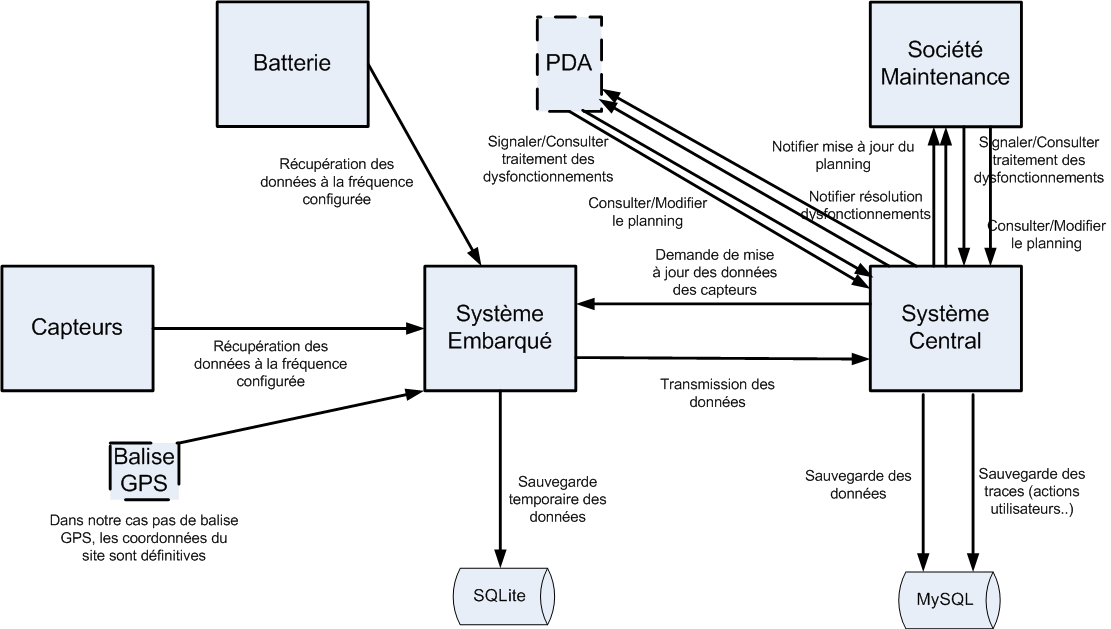
\includegraphics[width = \textwidth] {./img/Cas_Normal.png}
Ce schéma essaye de mettre en évidence l'ensemble des interactions ayant lieu dans un fonctionnement normal.

    \subsection{Scenarii Exceptionnels}

            \subsubsection{Alerte au système central}
            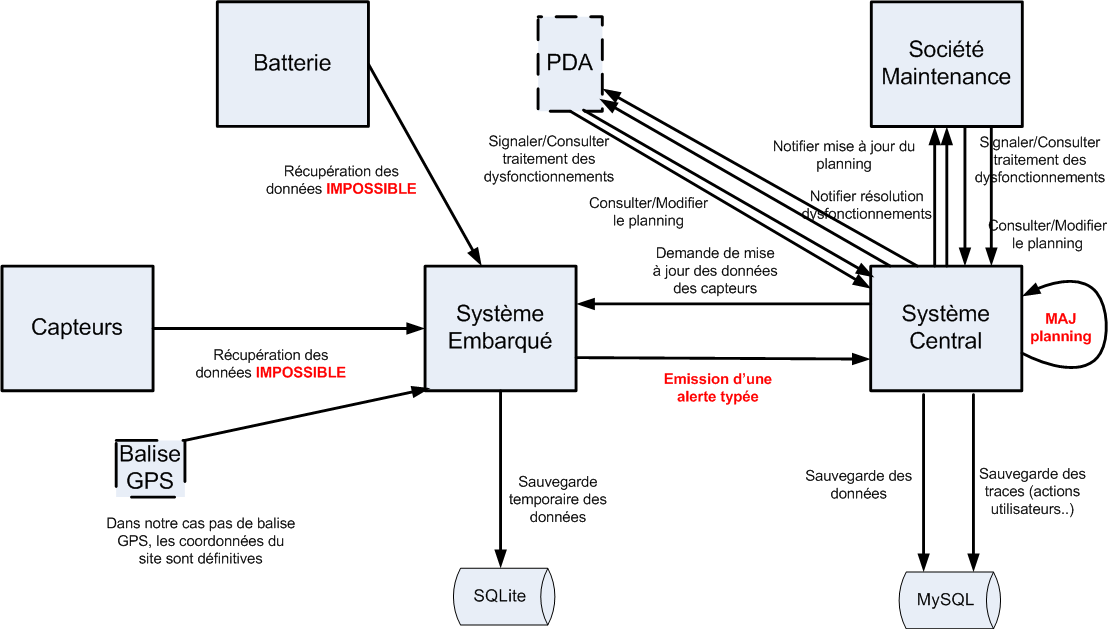
\includegraphics[width = \textwidth] {./img/Alertes.png}
Ce schéma met en évidence les traitements effectués quand le système embarqué détecte un dysfonctionnement.

            \subsubsection{Communication interrompu entre sites générique et central}
            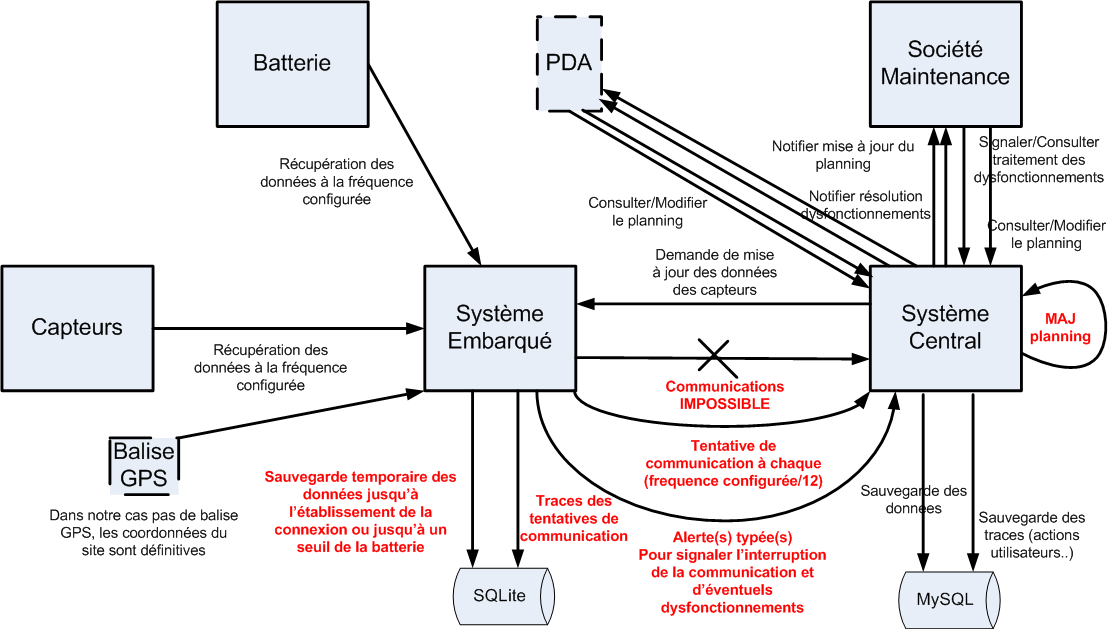
\includegraphics[width = \textwidth] {./img/CommunicationInterrompue.png}
Ce schéma met en évidence les traitements effectués quand le système embarqué n'arrive plus à communiquer 
avec le système central.

On peut imaginer un cas catastrophe ou les communications ne se rétablissement pas et que d'autres problèmes différents de celui de sauvegarde surviennent, par exemple que l'état des batteries soient critiques ou qu'une cuve soit pleine. Dans un souci de zéro défaut, on propose les solutions suivantes sans apporter plus de détails :
 \begin{description}
        \item[État critique de la batterie :] A partir d'un seuil, le système embarqué arrête de récolter les données (des capteurs, de la batterie et de la balise), et s'éteigne afin d'éviter des pertes de données durant son fonctionnement.
        \item[État critique niveau batterie :] On peut imaginer que le système embarqué soit relié à des actionneurs qui permettent d'ouvrir et fermer une vanne; cette vanne pourrait être une vanne d'évacuation pour diminuer le contenu d'une cuve ou ravitailler une cuve.
\end{description}
            \subsubsection{Maintenance à distance}
            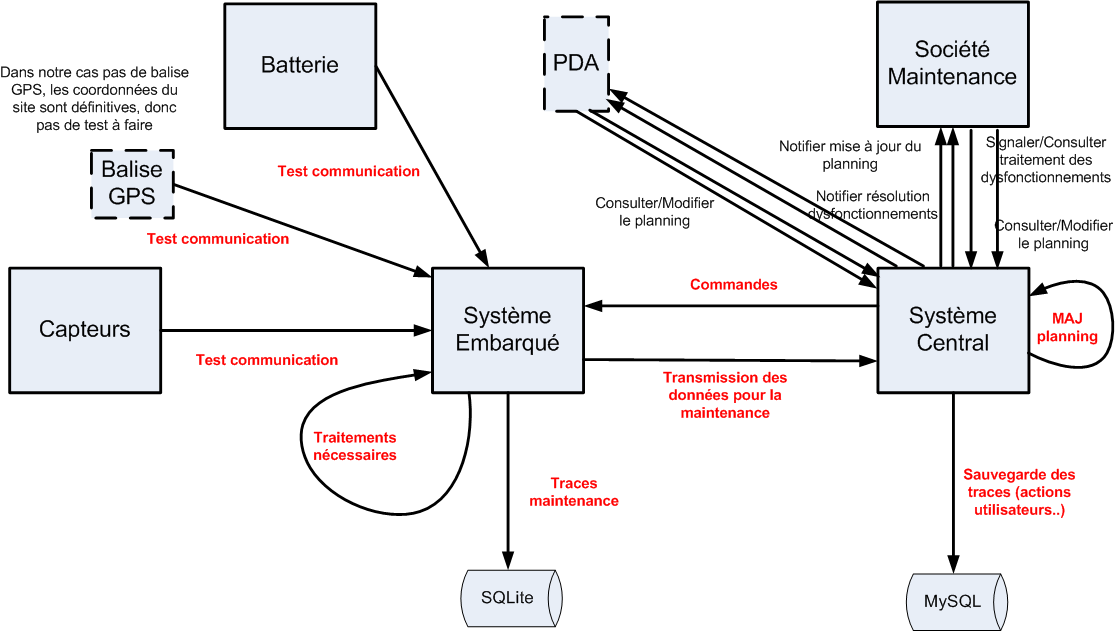
\includegraphics[width = \textwidth] {./img/MaintenanceDistante.png}
Ce schéma met en évidence les traitements effectués quand le système embarqué est maintenu à distance. Les commandes de maintenance seront 
très variées :
\begin{enumerate}
       \item Réinitialiser le système
       \item Vérifier les communications du système avec les capteurs, la source d'énergie, la balise GPS s'il y en a une.
       \item Faire une capture de l'état du système
       \item Tester les protocoles de communication (GPRS, Sattelite, d'autres s'ils en existent..).
 \end{enumerate}


\end{document}
